%=================================================================
\section{Introduction}
\label{sec-intro}

With all of the tweets circulating every second it is hard to tell whether the sentiment behind a specific tweet
 will impact a company, or a person's, brand for being viral (positive), or devastate profit because it strikes a 
 negative tone. Capturing sentiment in language is important in these times where decisions and reactions are
  created and updated in seconds. But, which words actually lead to the sentiment description? In this competition 
  you will need to pick out the part of the tweet (word or phrase) that reflects the sentiment.

Help build your skills in this important area with this broad dataset of tweets. Work on your technique 
to grab a top spot in this competition. What words in tweets support a positive, negative, or neutral sentiment? 
How can you help make that determination using machine learning tools?

In this competition we've extracted support phrases from Figure Eight's Data for Everyone platform. 
The dataset is titled Sentiment Analysis: Emotion in Text tweets with existing sentiment labels, 
used here under creative commons attribution 4.0. international licence. Your objective in this competition 
is to construct a model that can do the same - look at the labeled sentiment for a given tweet and figure
 out what word or phrase best supports it.\\


















\section{Data Exploratory Analysis } \label{sec-preliminaries}

Now let's take a look at the training data provided by this competition 
and do some exploratory data analysis to get a detailed understanding of the training set.\\
\begin{center}
  \begin{minipage}{1.2\linewidth}
  \centering
  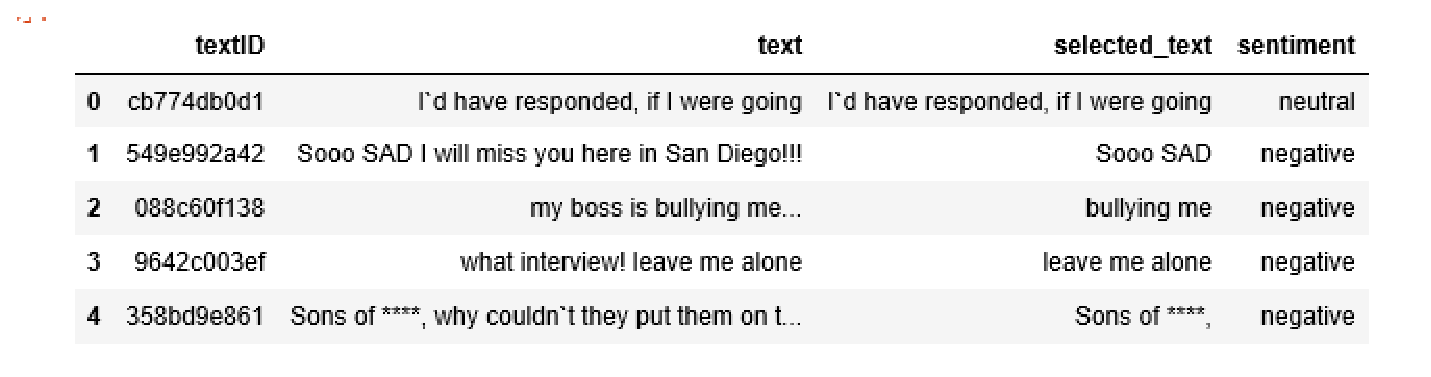
\includegraphics[width=1.2\textwidth]{kaggle/01.1.eps}
  {\small{Flag.1}}
  \end{minipage}
  \hfill
  \\
\end{center}
(1) Text and selected_text of one record in training set are null, 
so delete this data. \\
(2)
Check the distribution of the sentiment category in the training set data.
\begin{center}
  \begin{minipage}{1\linewidth}
    \centering
    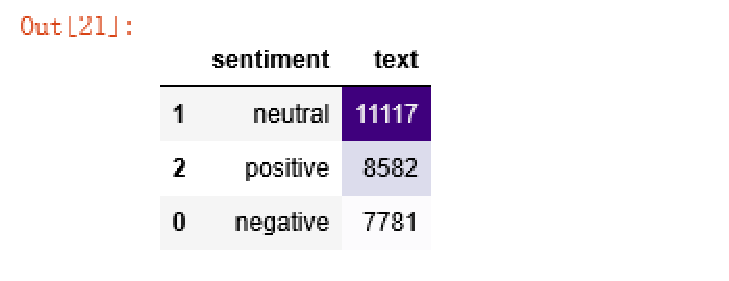
\includegraphics[width=1\textwidth]{kaggle/01.3.eps}
    {\small{Flag.2}}
    \end{minipage}
  \hfill
  \\
  We can see that across the entire dataset, there are 111,117 tweets for 
  neutral emotions, 8,582 tweets for positive emotions, and 7,781 tweets
   for negative emotions.
   \\
   
\end{center}

(3)Look at the Jaccard similarity between Text and selected_text.
\begin{center}
  \begin{minipage}{1\linewidth}
  \centering
  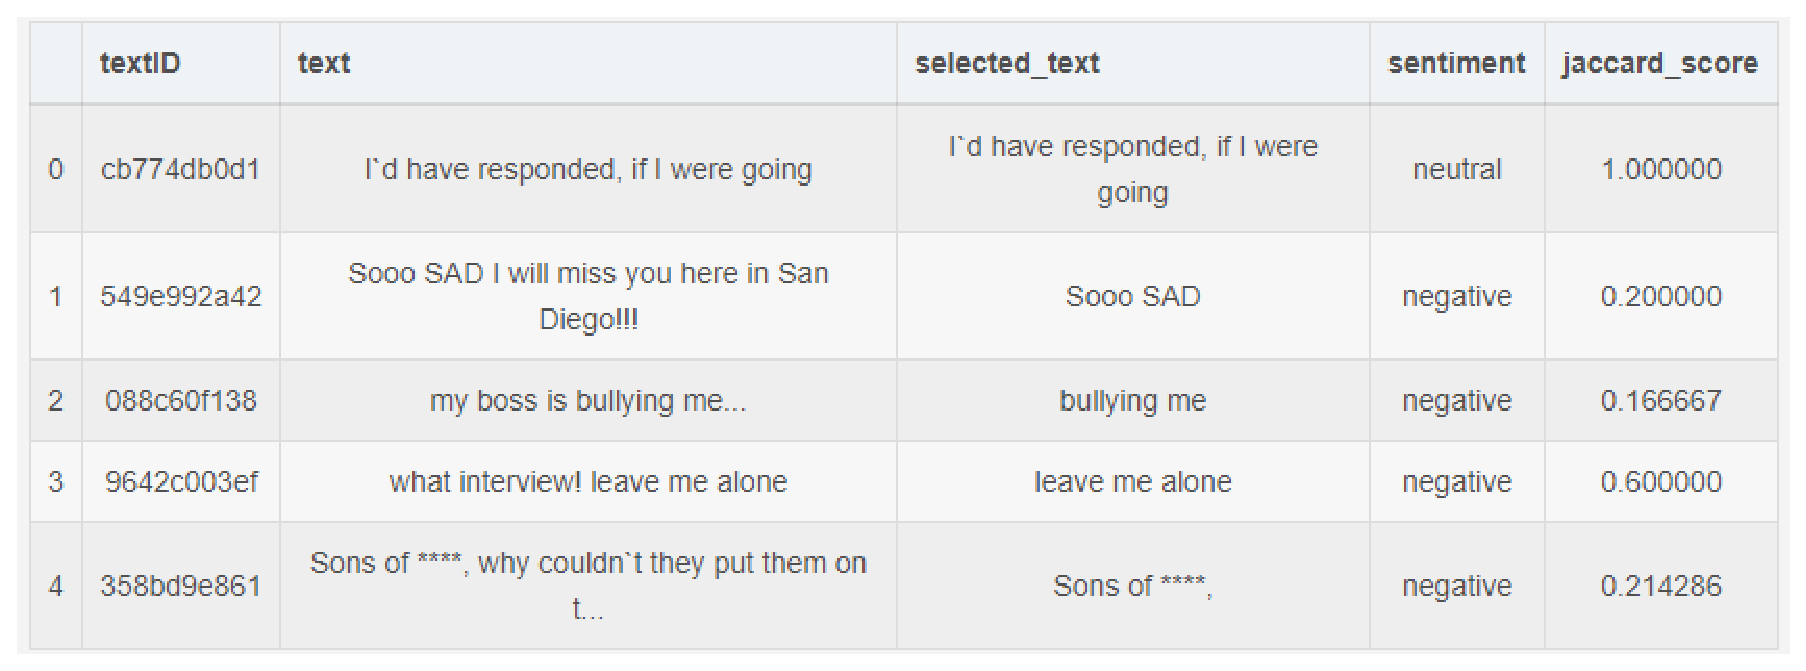
\includegraphics[width=1\textwidth]{kaggle/1.8.eps}
  {\small{Flag.3}}
  \end{minipage}
  \hfill
  \\
  As can be seen from the above output results,such as I`d have responded, if I 
  were going,This kind of words has the highest similarity with his
   emotional polarity, with a similarity value of 1, followed by words 
   like leave me alone, with a negative emotional polarity, with a 
   similarity value of 0.6.
\end{center}
(4)The kernel distribution graph of word length.

\begin{center}
  \begin{minipage}{0.4\linewidth}
  \centering

  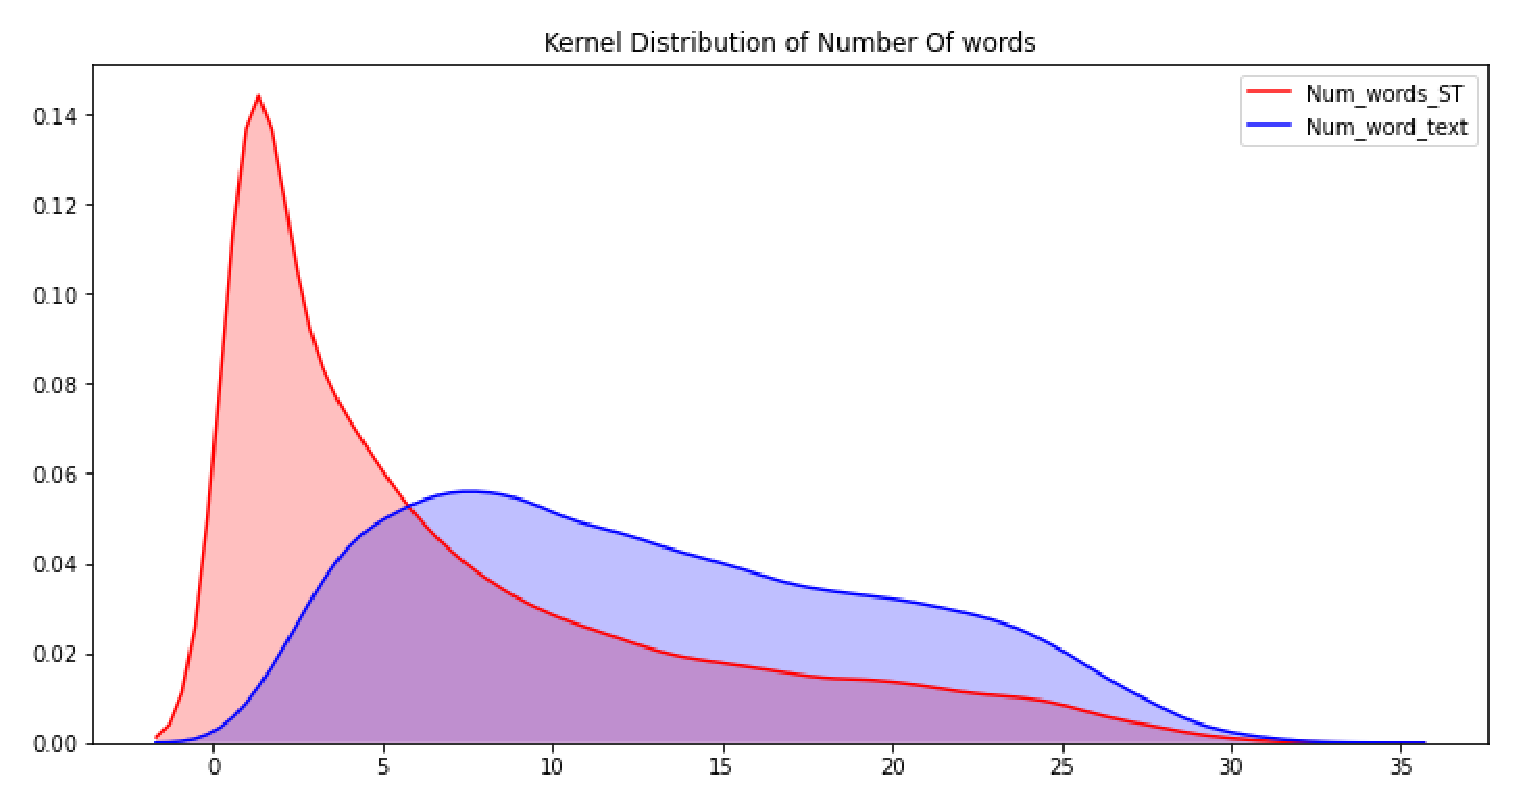
\includegraphics[width=0.9\textwidth]{kaggle/1.1.eps}
 
  {\small{Flag.4}}

  \end{minipage}
  \begin{minipage}{0.4\linewidth}
    \centering
  
    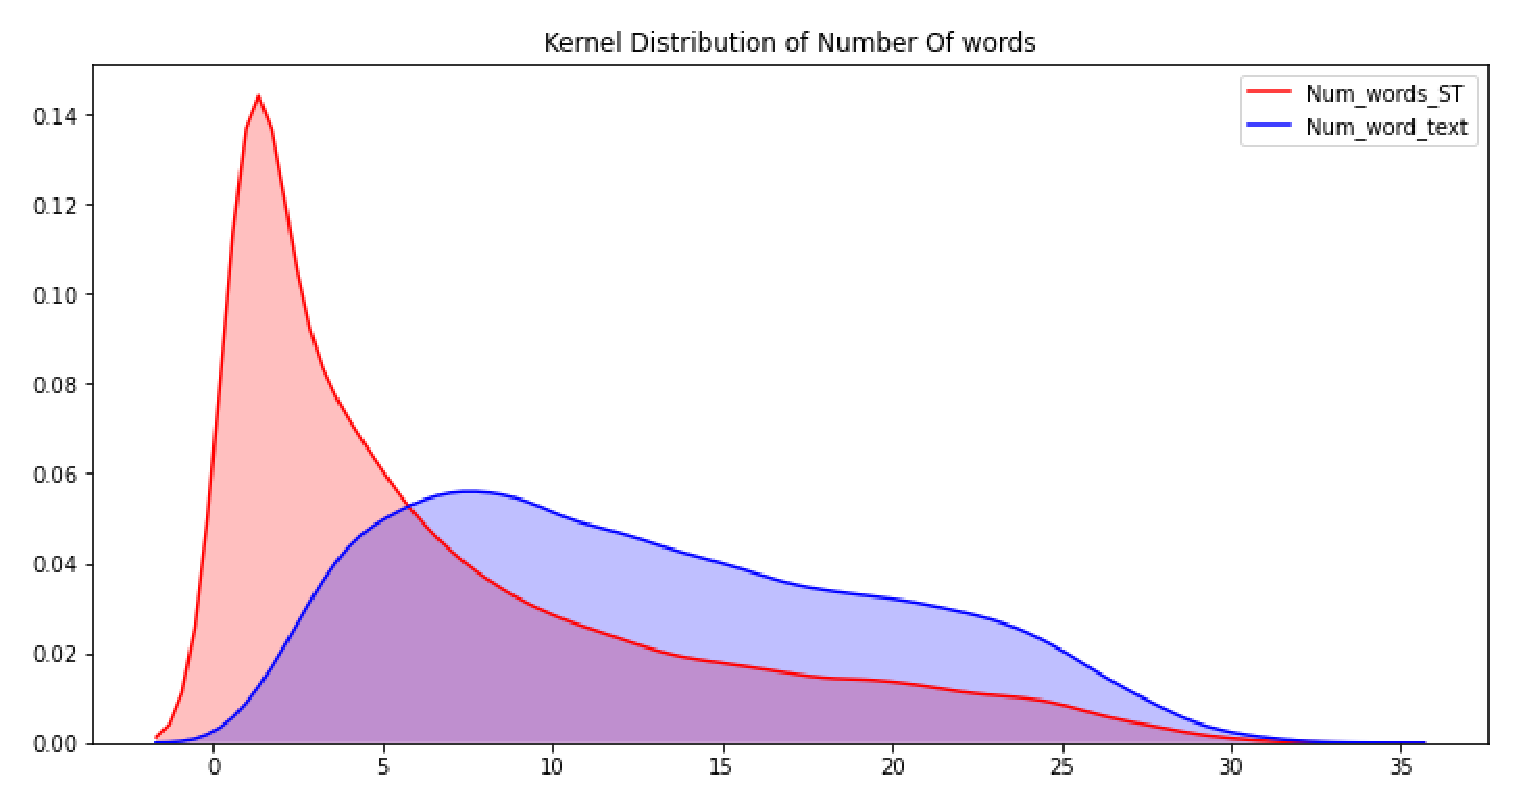
\includegraphics[width=0.9\textwidth]{kaggle/1.2.eps}
   
    {\small{Flag.5}}
  
    \end{minipage}
    \begin{minipage}{0.4\linewidth}
      \centering
    
      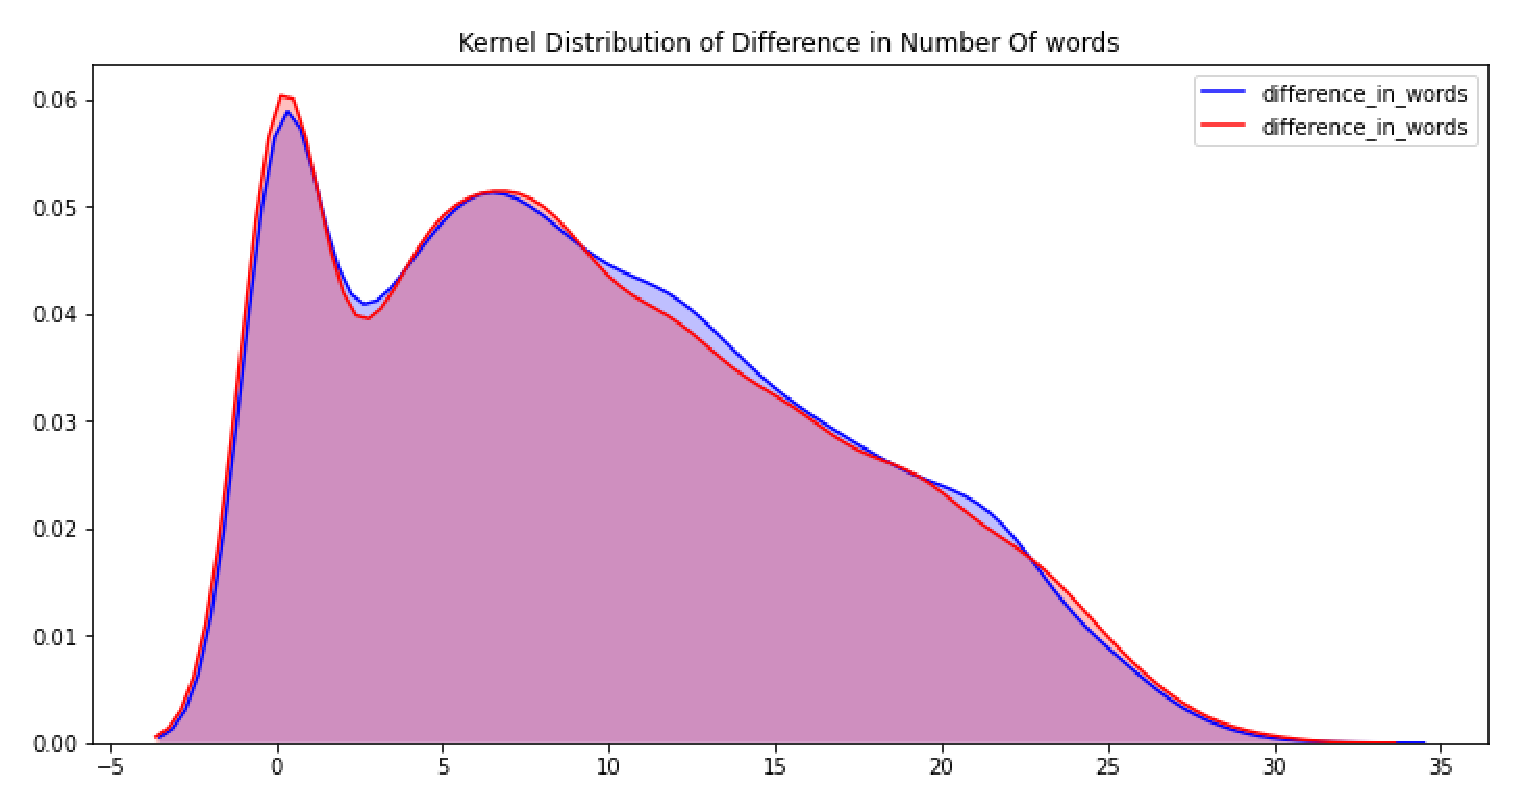
\includegraphics[width=0.9\textwidth]{kaggle/1.3.eps}
     
      {\small{Flag.6}}
    
      \end{minipage}
  \hfill
  ~\\
  The above three pictures are text and selected_text, respectively. The 
  kernel distribution picture of Jaccard similarity for Sentiment 
  classified as positive or negative word length difference.As can be 
  seen from the above figure, the Jaccard similarity of positive or 
  negative text and selected_text has two sharp kurtosis around 1.0 or
   0.1.The word length difference also has two kurtosis, where the 
   difference of 0 is a sharp kurtosis.That means that a large 
   percentage of positive or negative text is the same as selected_text.
\end{center}
(5)
The word cloud shows how often words appear in different categories of Twitter.
\begin{center}
  \begin{minipage}{0.5\linewidth}
  \centering

  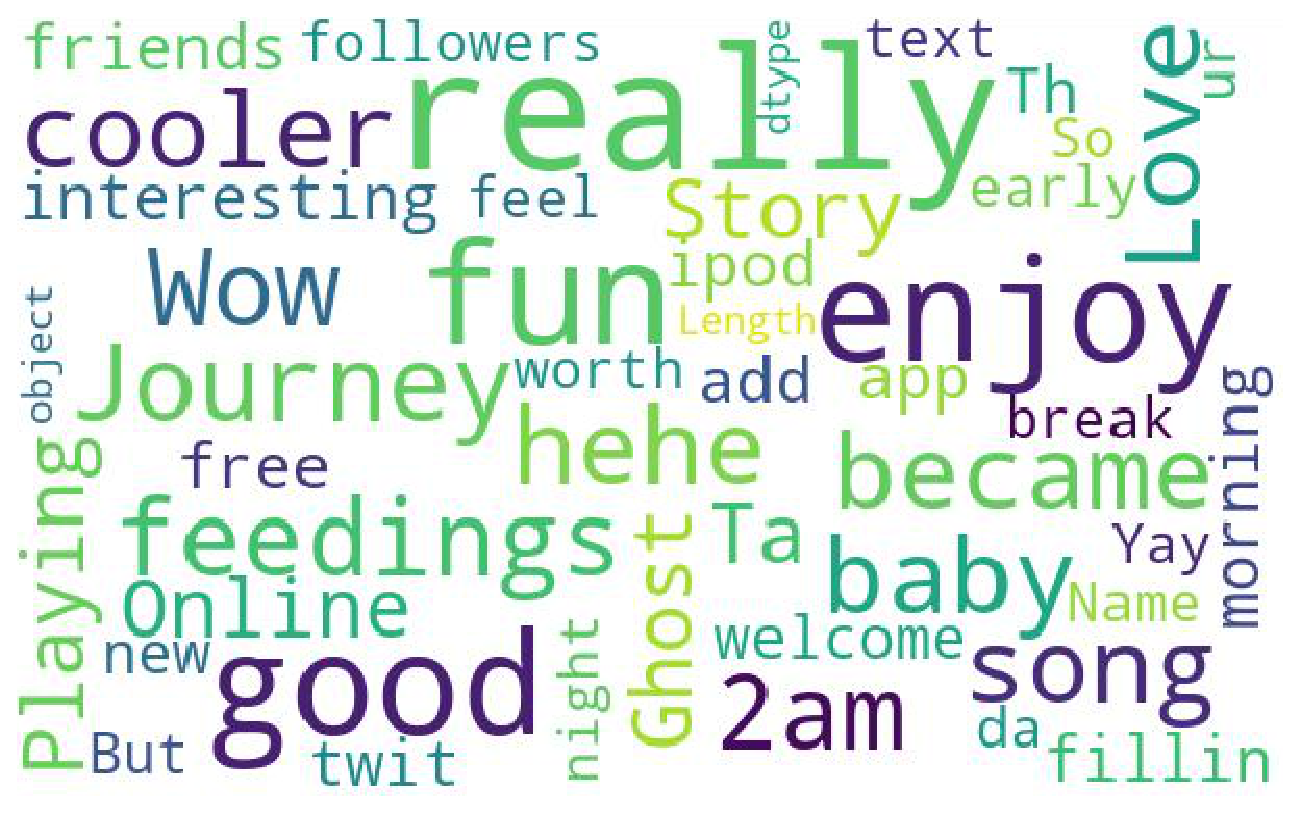
\includegraphics[width=1\textwidth]{kaggle/1.4.eps}
 
  {\small{Flag.8}}

  \end{minipage}
  \begin{minipage}{0.5\linewidth}
    \centering
  
    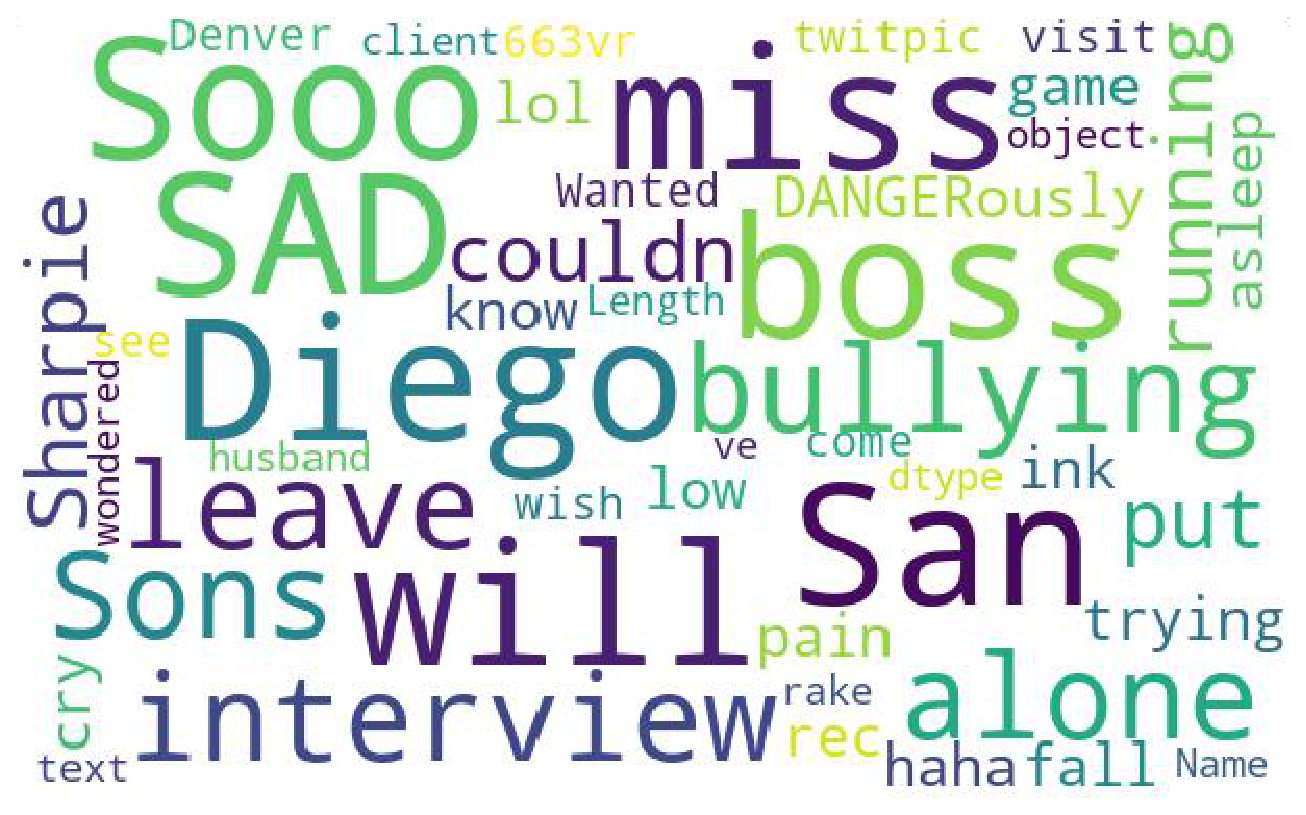
\includegraphics[width=1\textwidth]{kaggle/1.5.eps}
   
    {\small{Flag.9}}
  
    \end{minipage}
    \begin{minipage}{0.5\linewidth}
      \centering
      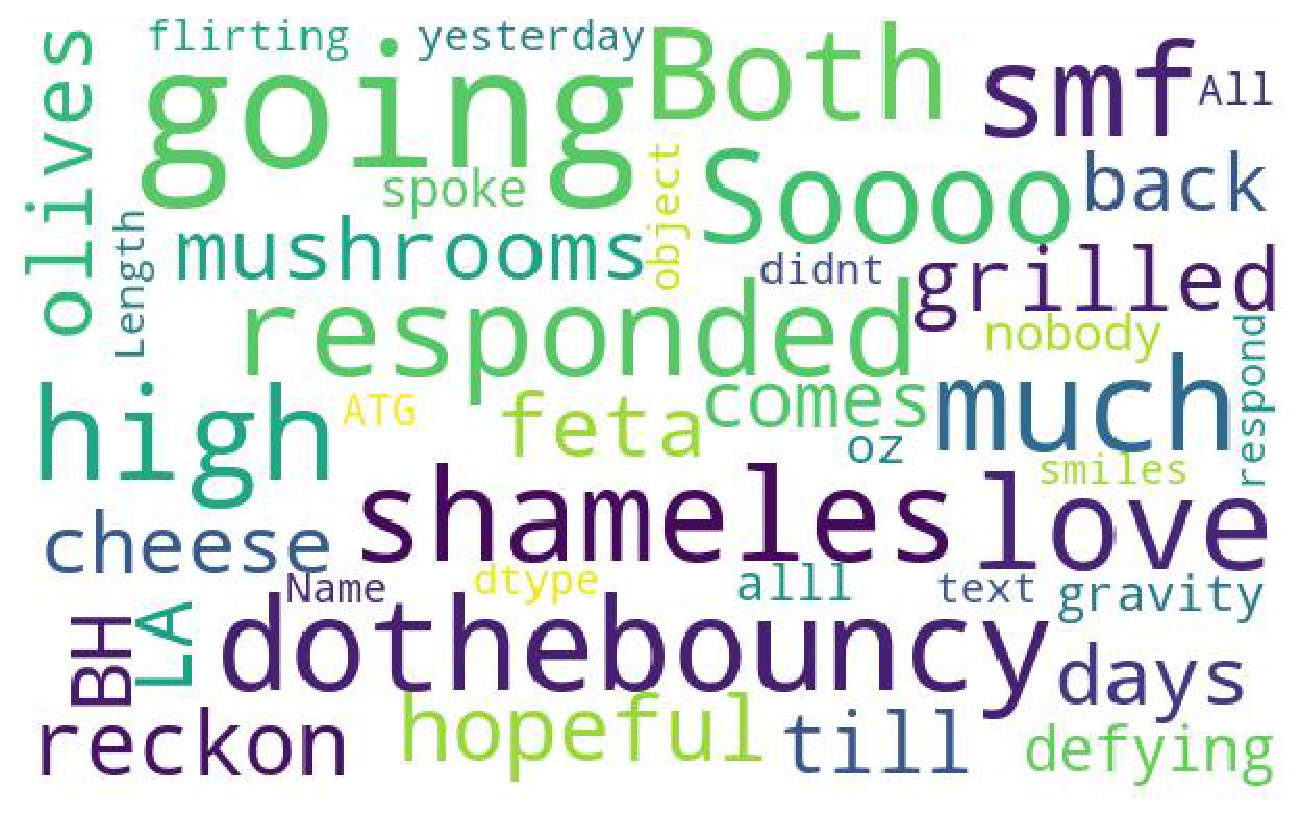
\includegraphics[width=1\textwidth]{kaggle/1.6.eps}
     
      {\small{Flag.10}}
      \end{minipage}
  \hfill
  ~\\
  The three word clouds show the most frequently used words in tweets
   for each of the three E-polarities.
For example, we can clearly see that we usually use words like happy, 
good and so on to express our happy mood, and these words are also 
obvious in our output word cloud.
\end{center}
\section{Model Construction and Training} 


These models for training in the large-scale corpus, it concluded that the word 
vector can be used in different field of NLP, but all of these training requires
 a lot of GPU, for the average person is unable to afford the cost of theraining
  from the start, so we can use has trained model parameters, used after 
  fine-tuning in our NLP tasks.Here I used Huggingface's open source Transformers 
  library, which provides a lot of pre-trained models with a very good and 
  easy-to-use interface that can be directly called and built using PyTorch or
   TensorFlow.

\begin{itemize}
  \item Construct tokenizer, and transform the text of training set and test set into token.
  ~\\By making a full connection layer of 768x1 to the output vector to get the Head,
   the output becomes the vector of BatchxMAX_LENx1, then rehaspe is the vector of
    BatchxMAX_LEN, and then Softmax.
\end{itemize}

\begin{itemize}
  \item Divide the training set into 5 copies, and take 4 copies of training and 1 copy for verification.
  \item Three epochs are trained each time, and parameters of the epoch with the lowest Loss in verification set are taken.We get a new model at the end of each training session, so we end up with 5 models.
  \item When making predictions, the prediction results of these five models will be averaged.
  \item The predicted values of the five trained models were averaged.
\end{itemize}
\begin{center}
  \begin{minipage}{1\linewidth}
  \centering
  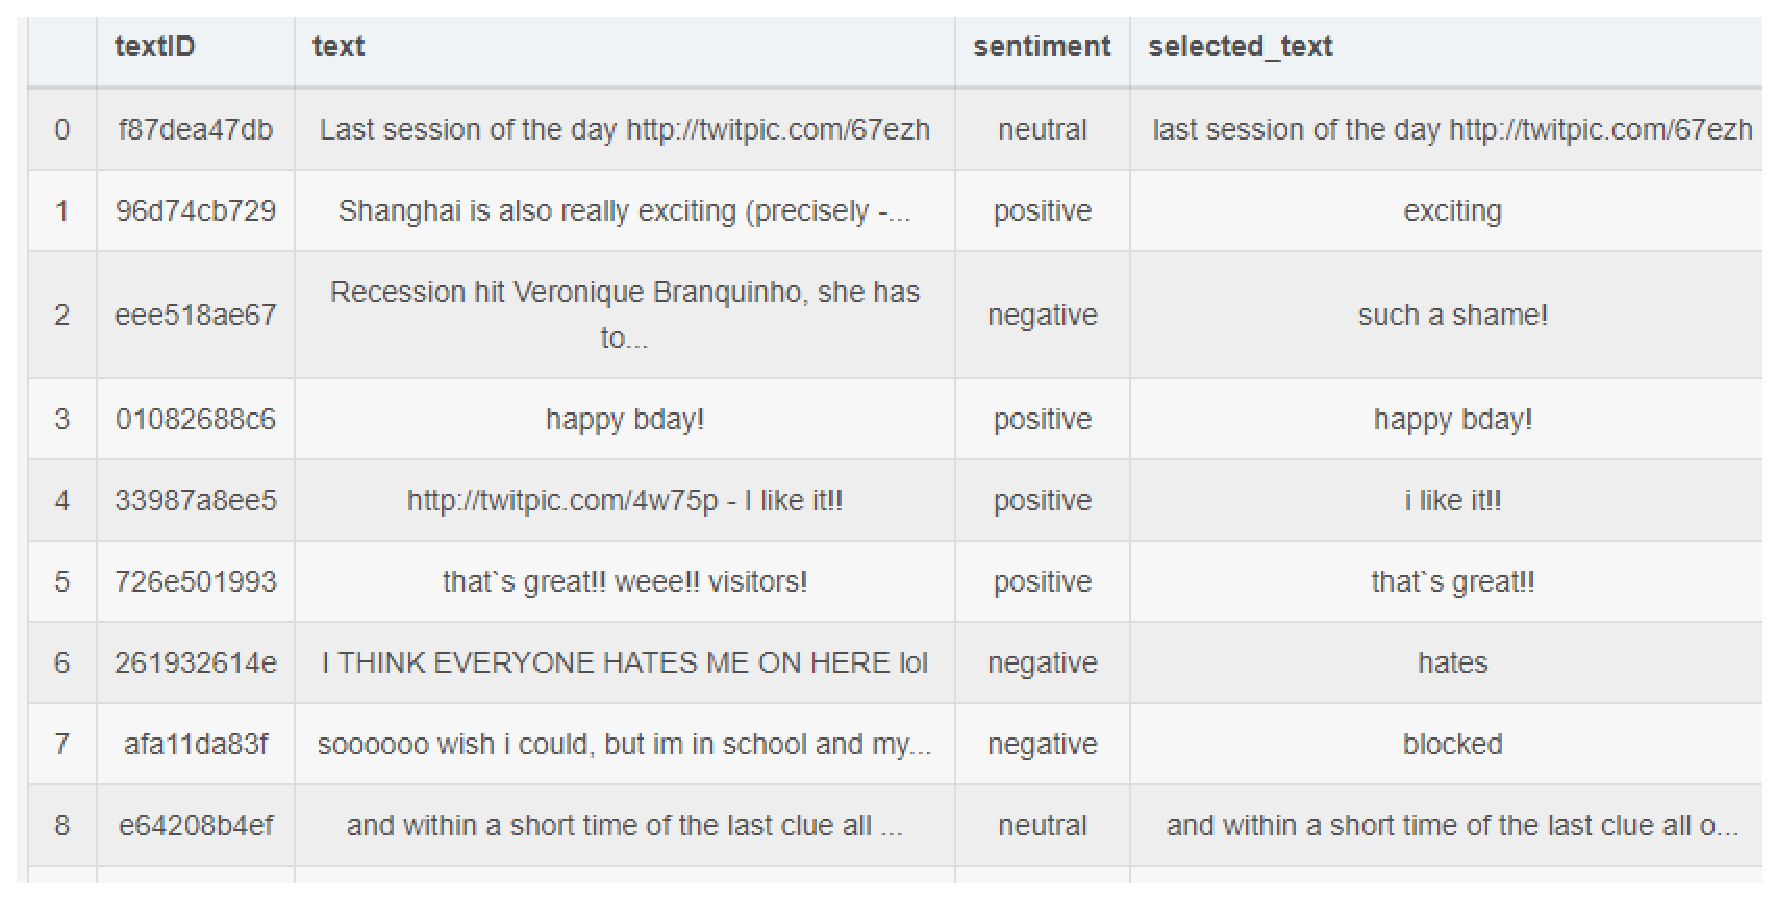
\includegraphics[width=1\textwidth]{kaggle/1.7.eps}
  {\small{Flag.11}}
  \end{minipage}
  \hfill
  \\

  
\end{center}

\section{Conclusions}

Through this project, we further understand the related contents of
 big data analysis, and also have a preliminary understanding of natural
  language processing. I believe this project experience will be of 
  great help in the following study.